\documentclass[12pt,onecolumn]{article}
\usepackage[utf8]{inputenc}
\usepackage{amsmath}
\usepackage{amssymb}
\usepackage{mathtools}
\usepackage{graphicx}
\usepackage{booktabs}
\usepackage{cite}
\usepackage{hyperref}
\usepackage{geometry}
\usepackage{algorithm}
\usepackage{algpseudocode}
\usepackage{setspace}
\usepackage{subcaption}
\usepackage{microtype}
\usepackage{tabularx}

\geometry{a4paper, margin=1in}
\onehalfspacing

\hypersetup{
    colorlinks=true,
    linkcolor=blue,
    citecolor=blue,
    urlcolor=blue
}

\title{\textbf{Mathematical Modeling and Performance Analysis of Multi-Node Queueing Networks Under Adversarial Attacks and Timeout-Driven Retransmissions}}
\author{
    \textbf{Ilias Chrysovergis}\thanks{Department of Electrical and Electronic Engineering, Imperial College London, London SW7 2AZ, UK, and Metatopia. Corresponding author: \texttt{ilias@chrysovergis.gr}}
}
\date{\today}

\begin{document}

\maketitle

\begin{abstract}
The reliable transport of data through adversarial networks requires a rigorous mathematical understanding of the coupled dynamics between malicious disruption and transport-layer recovery protocols. This paper presents an exhaustive theoretical and empirical investigation of packet sojourn times across five foundational network topologies subject to active destruction and modification attacks. By synthesizing classical queueing theory, renewal-reward theory, and fixed-point traffic conservation, we formulate closed-form and semi-analytical models for: (i) single-node pre-service destruction attacks with backoff, (ii) single-node post-service modification attacks, (iii) multi-hop tandem chains with hypoexponential moment matching, (iv) general $N$-node feedforward networks with stage-wise traffic attenuation and truncated delay expectations, and (v) $N$-node symmetric feedback meshes with Erlang-distributed path traversal. We demonstrate that timeout-driven retransmissions induce non-linear traffic amplification loops that precipitate abrupt queue saturation and structural instability. The theoretical models are validated against discrete-event simulations, demonstrating close agreement across all operational regimes with relative errors consistently below 2\% (and strictly under 0.30\% across all multi-node topologies).
\end{abstract}

\begin{figure}[t]
    \centering
    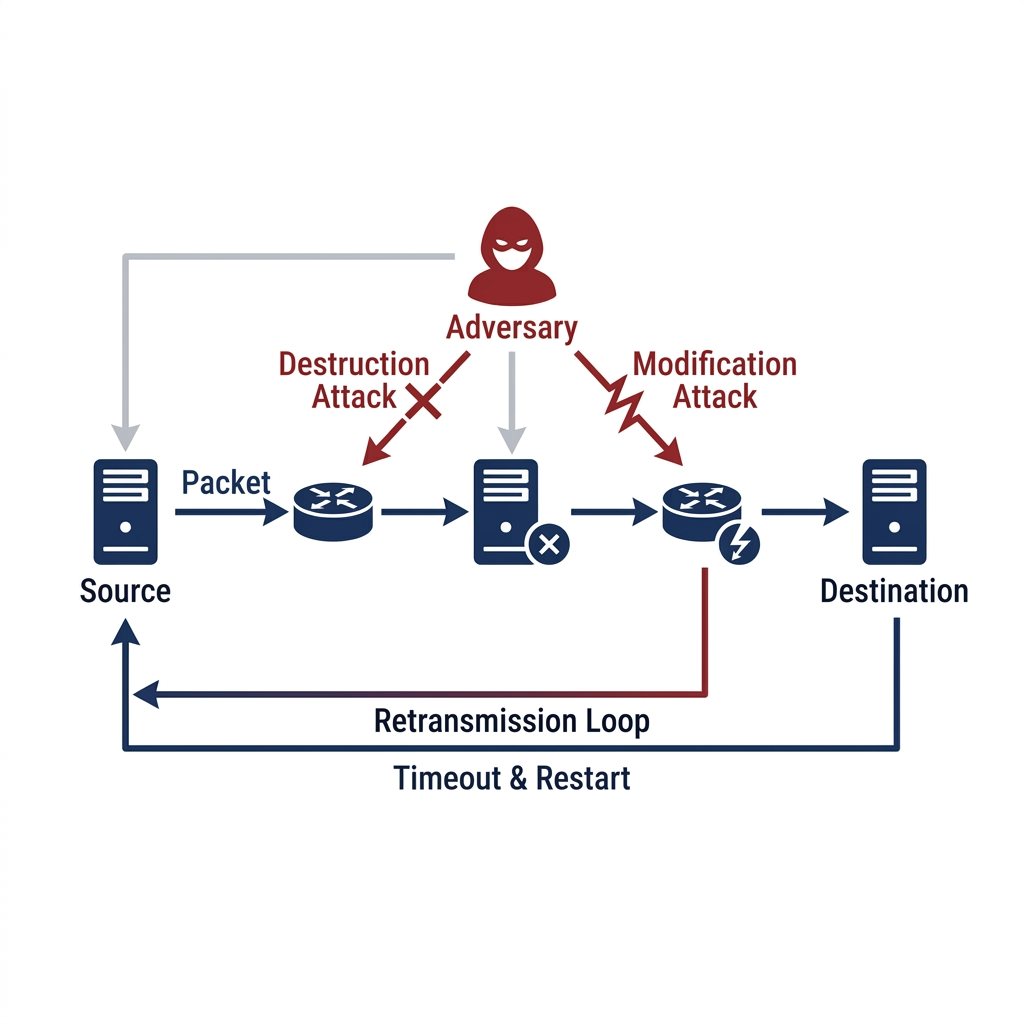
\includegraphics[width=0.85\textwidth]{fig1_system_model.png}
    \caption{Universal system model: Packets enter the network under external arrival rate $\lambda$. Nodes process packets at service rate $\mu$. Adversaries execute pre-service destruction or post-service modification attacks with probability $p$. Failures or timeout expiration ($>W$) trigger origin-based retransmissions, creating an amplified internal traffic stream $\Lambda^*$.}
    \label{fig:system_model}
\end{figure}

\section{Introduction}
Modern distributed architectures—ranging from wireless sensor swarms and Internet of Things (IoT) deployments to multi-hop tactical communications—frequently operate in hostile environments where communication links are unreliable and actively contested by malicious adversaries \cite{wood2002denial, pelechrinis2011denial}. Traditional queueing frameworks (such as Jackson networks \cite{jackson1957networks} or standard $M/M/1$ queues \cite{kleinrock1975queueing}) assume benign stochastic environments and complete packet conservation. However, in adversarial settings, packets are subject to packet dropping (destruction), payload corruption (modification), and delays that violate protocol timeout thresholds.

To guarantee eventual packet delivery, transport protocols employ automatic repeat request (ARQ) mechanisms governed by timeout deadlines \cite{fall1996simulation}. While timeout-driven retransmissions ensure reliable delivery, they introduce a powerful \textit{positive feedback loop}:
\begin{align*}
\text{Attacks / Delay} &\implies \text{Timeouts / Retransmissions} \\
&\implies \text{Increased Total Traffic } \Lambda^* \\
&\implies \text{Severe Congestion} \implies \text{Further Timeouts.}
\end{align*}
This feedback mechanism leads to sharp "cliff-edge" instability thresholds where a minor increase in the external arrival rate $\lambda$ or attack probability $p$ causes queue lengths and packet delay to diverge to infinity.

In this paper, we develop a unified, comprehensive theoretical foundation to model end-to-end sojourn times and stability boundaries across five distinct case studies. The remainder of this paper is organized as follows:
\begin{itemize}
    \item \textbf{Section 2} formalizes the general renewal-reward framework, traffic conservation fixed points, and base $M/M/1$ queueing relationships.
    \item \textbf{Section 3} analyzes single-node systems under two distinct threat models: pre-service destruction (Case 1) and post-service modification (Case 2).
    \item \textbf{Section 4} expands the theory to multi-hop feedforward topologies, analyzing 3-node tandem chains (Case 3) and general $N$-node chains with stage attenuation and truncated Gamma delay expectations (Case 4).
    \item \textbf{Section 5} formulates the theory for $N$-node symmetric feedback meshes (Case 5) using Jackson network routing and Erlang-$k$ visit summations.
    \item \textbf{Section 6} synthesizes the comparative theoretical properties across all topologies.
    \item \textbf{Section 7} presents validation against discrete-event simulations.
    \item \textbf{Section 8} establishes the Saddle-Node (Fold) retry bifurcation and critical collapse theory.
    \item \textbf{Section 9} concludes the paper.
\end{itemize}

\section{Universal Mathematical Framework}
\subsection{Renewal-Reward Model of Retransmissions}
Consider a packet arriving externally to a queueing network at rate $\lambda$. The journey of each packet comprises a sequence of independent and identically distributed (i.i.d.) transmission attempts. An attempt succeeds if the packet traverses the designated path without encountering an adversarial attack and without exceeding the timeout threshold $W$.

Let $P_{\text{succ}}$ denote the probability that an attempt succeeds, and let $P_{\text{fail}} = 1 - P_{\text{succ}}$ denote the failure probability. The total number of transmission attempts $A$ required for successful delivery is a geometric random variable with parameter $P_{\text{succ}}$:
\begin{equation}
P(A = a) = (1 - P_{\text{succ}})^{a-1} P_{\text{succ}}, \quad a \in \{1, 2, 3, \dots\}
\end{equation}
The expected number of attempts is:
\begin{equation}
E[A] = \frac{1}{P_{\text{succ}}}
\end{equation}
Each packet undergoes $A - 1$ failed attempts followed by exactly one successful attempt. Applying the renewal-reward theorem, the total end-to-end sojourn time $D$ is:
\begin{equation}
E[D] = (E[A] - 1) E[D_{\text{fail}}] + E[D_{\text{succ}}] + (E[A] - 1) B
\label{eq:general_delay}
\end{equation}
where $E[D_{\text{fail}}]$ is the expected duration of a failed attempt, $E[D_{\text{succ}}]$ is the expected duration of the final successful attempt, and $B \ge 0$ is a deterministic retransmission backoff delay.

\subsection{Fixed-Point Traffic Conservation}
Because every failed attempt generates a retransmission, the total effective arrival rate $\Lambda^*$ entering the network exceeds the external arrival rate $\lambda$. By traffic conservation:
\begin{equation}
\Lambda^* = \lambda \cdot E[A](\Lambda^*) = \frac{\lambda}{P_{\text{succ}}(\Lambda^*)}
\label{eq:fixed_point_general}
\end{equation}
Equation \eqref{eq:fixed_point_general} is a non-linear mean-field fixed-point equation in $\Lambda^*$, equivalently expressed via the effective throughput conservation map $\Gamma(\Lambda^*) \triangleq \Lambda^* P_{\text{succ}}(\Lambda^*) = \lambda$ (or $\Lambda^* P_{\text{succ}}(\Lambda^*)/E[V](\Lambda^*) = \lambda$ in feedback meshes). Because $P_{\text{succ}}$ depends on the queueing delays (which are monotonically increasing functions of $\Lambda^*$), $P_{\text{succ}}(\Lambda^*)$ decreases monotonically with $\Lambda^*$, whereas $\Gamma(\Lambda^*)$ is unimodal on $(0, \Lambda_{\text{crit}})$. Under finite timeout $W < \infty$, two fixed points $\Lambda_{\text{stable}}^* < \Lambda_{\text{SN}}^* < \Lambda_{\text{unstable}}^*$ coexist for every subcritical arrival rate $\lambda < \lambda_{\text{crit}}^{\text{SN}} \triangleq \max_{\Lambda^* \in (0, \Lambda_{\text{crit}})} \Gamma(\Lambda^*)$, coalescing at the Saddle-Node fold $\Lambda_{\text{SN}}^*$ and satisfying the server saturation bound:
\begin{equation}
\Lambda_{\text{stable}}^* \le \Lambda_{\text{SN}}^* < \Lambda_{\text{crit}}
\end{equation}
where $\Lambda_{\text{crit}}$ is the topology-dependent internal server saturation limit.

\section{Single-Node Analytical Models}
We first evaluate an isolated server with service rate $\mu$ under two fundamentally different attack models.

\subsection{Case Study 1: Single-Node Pre-Service Destruction Attacks}
\subsubsection{Adversary and Protocol Model}
In a pre-service destruction attack, an adversary intercepts and destroys the packet before it receives service from the server (e.g., dropped at the head of the queue upon being selected for service) with probability $p$. If destroyed, the packet consumes no server processing time, but the time spent waiting in the queue is wasted, and the packet undergoes a deterministic backoff $B$ before re-entering the queue. If the packet is not attacked (probability $1 - p$), it enters the server and is processed with exponential service time $S \sim \text{Exp}(\mu)$. The timeout threshold $T$ is checked against the total service phase $(W_q + S)$.

\subsubsection{Queueing Dynamics and Effective Load}
Let $\Lambda^*$ be the total arrival rate of attempts at the queue. Because destroyed packets exit before occupying the server, only non-destroyed packets consume service capacity. The effective arrival rate processed by the server is:
\begin{equation}
\lambda_{\text{eff}} = \Lambda^*(1 - p)
\end{equation}
The server utilization is:
\begin{equation}
\rho = \frac{\lambda_{\text{eff}}}{\mu} = \frac{\Lambda^*(1 - p)}{\mu} < 1
\end{equation}
The system behaves as an $M/M/1$ queue with arrival rate $\lambda_{\text{eff}}$ and service rate $\mu$. The expected waiting time in queue $E[W_q]$ and expected service time $E[S]$ are:
\begin{equation}
E[W_q] = \frac{\rho}{\mu(1 - \rho)} = \frac{\Lambda^*(1 - p)}{\mu(\mu - \Lambda^*(1 - p))}, \quad E[S] = \frac{1}{\mu}
\end{equation}

\subsubsection{Timeout and Success Probability}
For an $M/M/1$ queue with effective clearance rate $\gamma = \mu - \lambda_{\text{eff}}$, the cumulative distribution function (CDF) of the total time in system $W_q + S \sim \text{Exp}(\gamma)$ for a surviving attempt is:
\begin{equation}
P(W_q + S \le t \mid \text{not attacked}) = 1 - e^{-\gamma t} = 1 - e^{-(\mu - \Lambda^*(1-p))t}
\end{equation}
A transmission attempt succeeds if and only if the packet is not attacked and completes service within the timeout window $T$:
\begin{equation}
P_{\text{succ}} = (1 - p) P(W_q + S \le T \mid \text{not attacked}) = (1 - p)\left(1 - e^{-(\mu - \Lambda^*(1-p))T}\right)
\end{equation}
The expected delay per attempt is the expected wait plus the service time (incurred only if not attacked):
\begin{equation}
E[D_{\text{attempt}}] = E[W_q] + (1 - p) E[S] = \frac{\Lambda^*(1-p)}{\mu(\mu - \Lambda^*(1-p))} + \frac{1-p}{\mu}
\end{equation}
The total end-to-end sojourn time is:
\begin{equation}
E[D] = E[A] E[D_{\text{attempt}}] + (E[A] - 1) B = \frac{1}{P_{\text{succ}}} \left[E[W_q] + \frac{1-p}{\mu}\right] + \left(\frac{1}{P_{\text{succ}}} - 1\right) B
\end{equation}
The equilibrium rate $\Lambda^*$ is obtained by iteratively solving $\Lambda^* = \lambda_n / P_{\text{succ}}(\Lambda^*)$.

\subsection{Case Study 2: Single-Node Post-Service Modification Attacks}
\subsubsection{Adversary and Protocol Model}
In a post-service modification attack, the adversary corrupts the packet payload during transmission. The node processes every packet fully ($S \sim \text{Exp}(\mu)$). The corruption is detected via checksum/integrity verification only \textit{after} service completion. Consequently, every attempt—successful or failed—occupies the server for a full service interval.

\subsubsection{Queueing Dynamics and Sojourn Time}
Because all attempts consume server capacity, the server arrival rate is the total rate $\Lambda^*$. The server utilization is:
\begin{equation}
\rho = \frac{\Lambda^*}{\mu} < 1
\end{equation}
The total time spent by a packet in the system during an attempt (queueing plus service) follows an exponential distribution with rate parameter $\gamma = \mu - \Lambda^*$:
\begin{equation}
f_S(t) = (\mu - \Lambda^*) e^{-(\mu - \Lambda^*) t}, \quad P(S \le T) = 1 - e^{-(\mu - \Lambda^*) T}
\end{equation}
The expected attempt duration is:
\begin{equation}
E[S] = \frac{1}{\mu - \Lambda^*}
\end{equation}

\subsubsection{Success Probability and Renewal Delay}
An attempt succeeds if it escapes adversarial corruption (probability $1 - p$) and finishes before timeout $T$:
\begin{equation}
P_{\text{succ}} = (1 - p) P(S \le T) = (1 - p)\left(1 - e^{-(\mu - \Lambda^*) T}\right)
\end{equation}
The expected number of attempts is $E[A] = 1/P_{\text{succ}}$. By renewal theory:
\begin{equation}
E[D] = E[A] \cdot E[S] = \frac{1}{(1 - p)\left(1 - e^{-(\mu - \Lambda^*) T}\right)(\mu - \Lambda^*)}
\end{equation}
The fixed-point traffic rate satisfies:
\begin{equation}
\Lambda^* = \frac{\lambda_n}{(1 - p)\left(1 - e^{-(\mu - \Lambda^*) T}\right)}
\end{equation}

\subsection{Theoretical Comparison: Destruction vs. Modification}
Comparing Case 1 and Case 2 highlights a fundamental queueing principle:
\begin{itemize}
    \item \textbf{Destruction Attacks (Case 1):} Server utilization depends only on surviving traffic $\Lambda^*(1-p)$. The system stability condition is $\Lambda^*(1-p) < \mu \implies \Lambda^* < \frac{\mu}{1-p}$. The adversary inadvertently unloads the server by dropping packets prior to service.
    \item \textbf{Modification Attacks (Case 2):} Server utilization is driven by the full attempt stream $\Lambda^*$. The stability condition is strictly $\Lambda^* < \mu$. Because corrupted packets waste full service cycles, modification attacks drive the queue to saturation at substantially lower external arrival rates $\lambda_n$.
\end{itemize}
This theoretical divergence is confirmed in Figure \ref{fig:single_node}.

\begin{figure}[h]
    \centering
    \begin{subfigure}[b]{0.48\textwidth}
        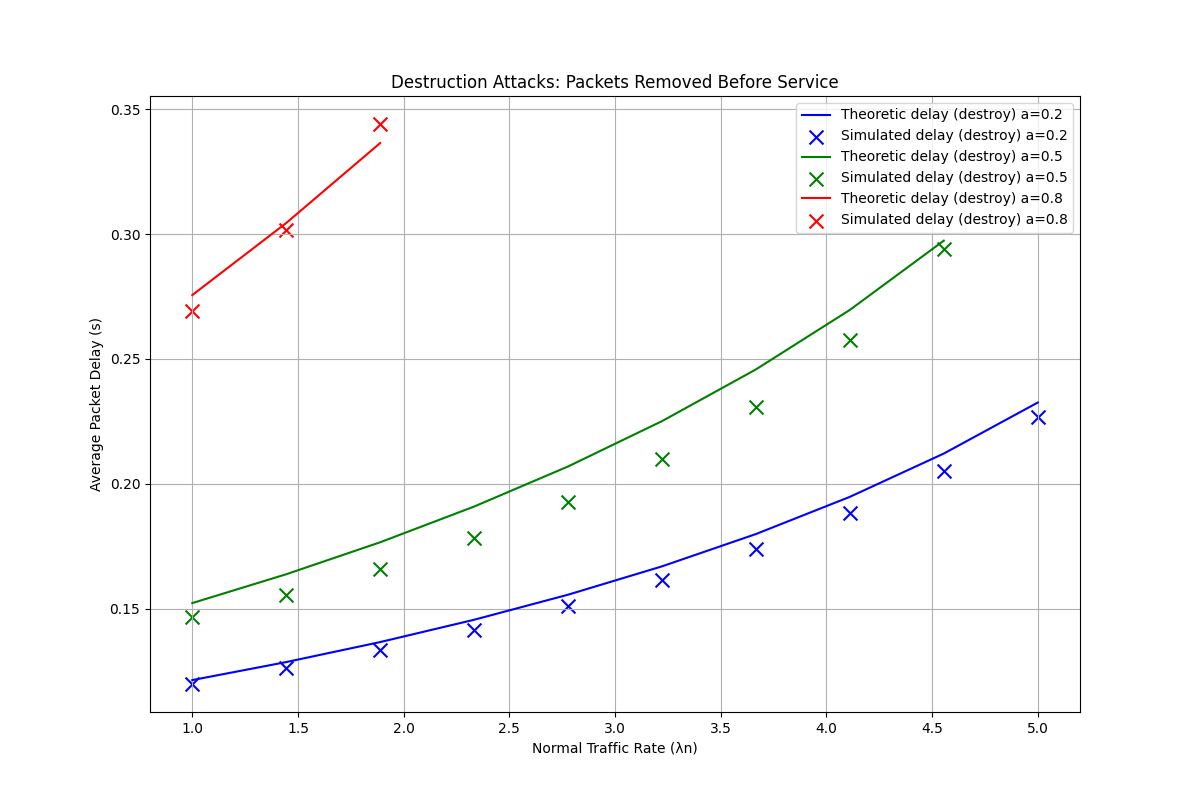
\includegraphics[width=\textwidth]{1_one_node_destruction/destroy_no_service_plot_reps200.png}
        \caption{Case 1: Pre-Service Destruction}
    \end{subfigure}
    \hfill
    \begin{subfigure}[b]{0.48\textwidth}
        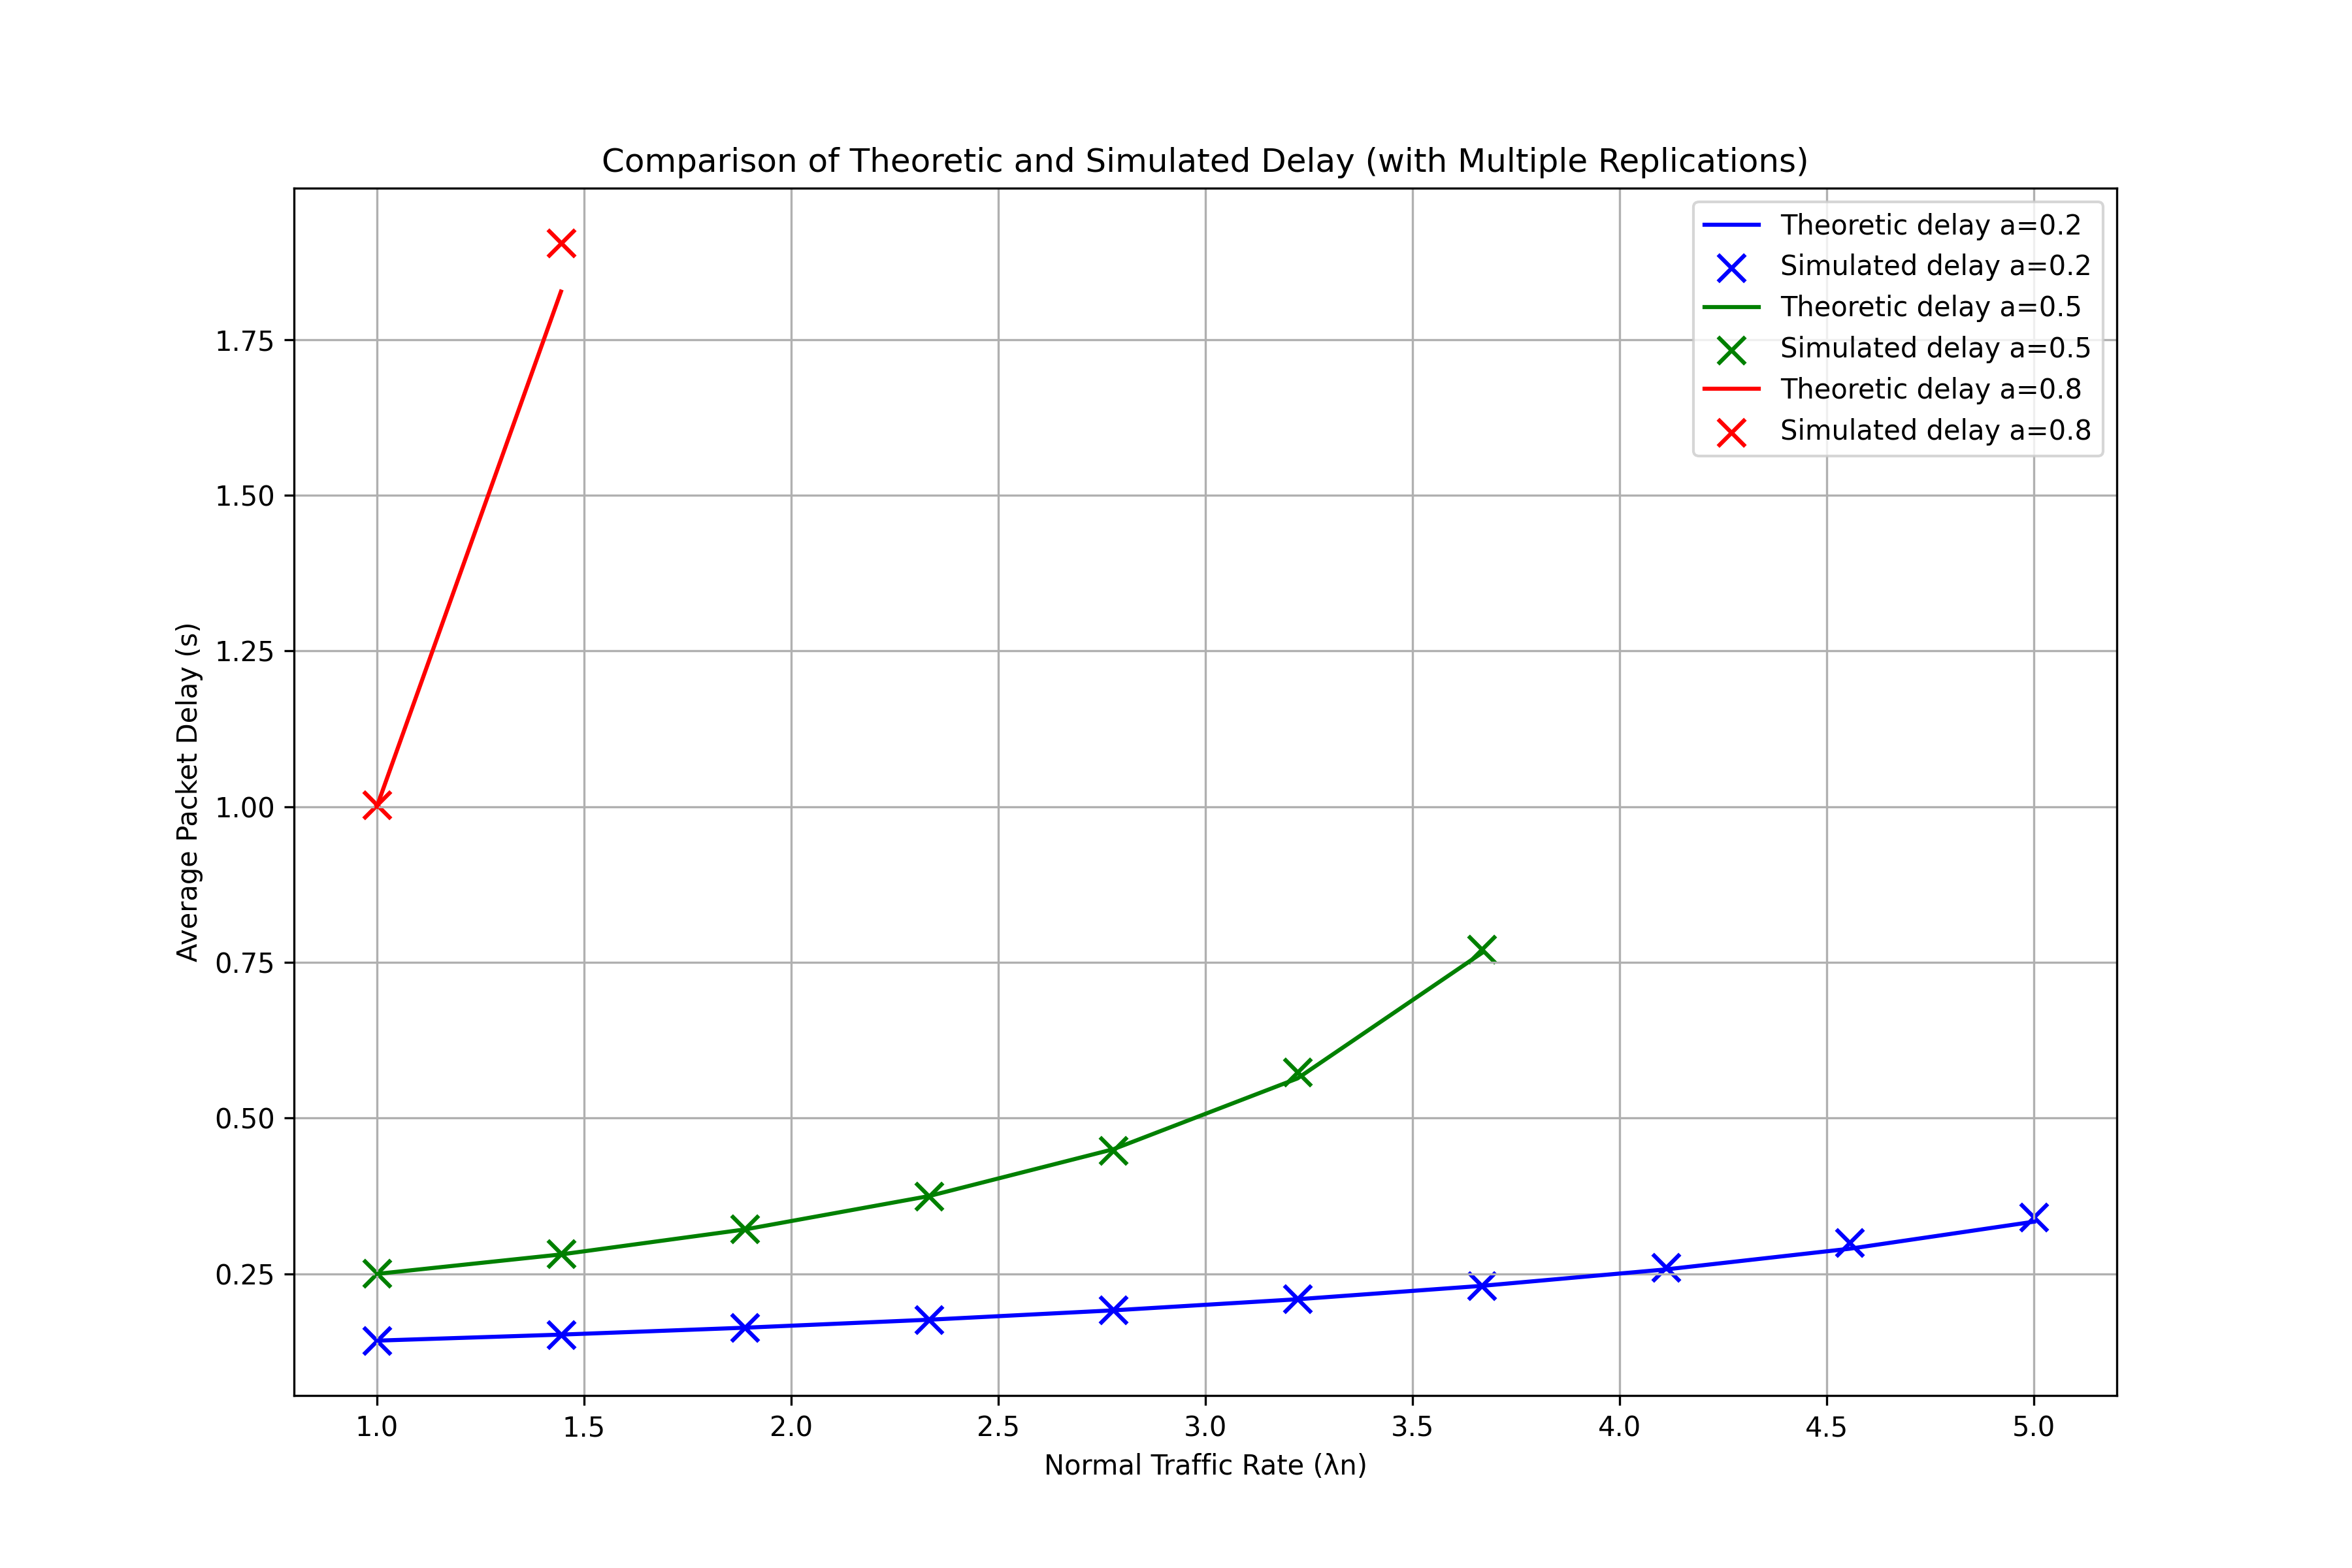
\includegraphics[width=\textwidth]{2_one_node_modification/plot_reps50_warmup500_sim5000.png}
        \caption{Case 2: Post-Service Modification}
    \end{subfigure}
    \caption{Single-node delay comparison. Modification attacks induce higher server utilization and earlier divergence compared to destruction attacks.}
    \label{fig:single_node}
\end{figure}

\section{Multi-Hop Feedforward Networks}
\subsection{Hypoexponential Journey Time \& Gamma Matching}
In a multi-hop feedforward network, a packet must traverse a sequence of $N$ distinct nodes in series: Node $0 \to \text{Node } 1 \to \dots \to \text{Node } (N-1)$. Let $\Lambda_j^*$ be the arrival rate at node $j$, and let $\mu_j = \mu$ be the service rate. By Burke's theorem~\cite{burke1956output} and Jackson network approximations~\cite{jackson1957networks, kleinrock1976computer}, each node $j$ operates as an $M/M/1$ queue with sojourn time $X_j \sim \text{Exp}(\mu - \Lambda_j^*)$:
\begin{equation}
E[X_j] = \frac{1}{\mu - \Lambda_j^*}, \quad \text{Var}(X_j) = \frac{1}{(\mu - \Lambda_j^*)^2}
\end{equation}
The total continuous journey time across $N$ nodes is the convolution of $N$ independent exponential random variables, known as a \textbf{Hypoexponential distribution}:
\begin{equation}
S_N = \sum_{j=0}^{N-1} X_j
\end{equation}
The exact mean and variance of $S_N$ are:
\begin{equation}
\mu_S = E[S_N] = \sum_{j=0}^{N-1} \frac{1}{\mu - \Lambda_j^*}, \quad \sigma_S^2 = \text{Var}(S_N) = \sum_{j=0}^{N-1} \frac{1}{(\mu - \Lambda_j^*)^2}
\end{equation}
Because the exact Hypoexponential CDF involves complex combinatorial sums of exponentials that become numerically unstable for large $N$, we employ a two-parameter \textbf{Gamma moment-matching approximation}~\cite{cox1955use, altiok1985approximate, ross1996stochastic} $S_N \sim \text{Gamma}(k, \theta)$ with shape $k$ and scale $\theta$:
\begin{equation}
k = \frac{\mu_S^2}{\sigma_S^2} = \frac{\left(\sum_{j=0}^{N-1} \frac{1}{\mu - \Lambda_j^*}\right)^2}{\sum_{j=0}^{N-1} \frac{1}{(\mu - \Lambda_j^*)^2}}, \quad \theta = \frac{\sigma_S^2}{\mu_S} = \frac{\sum_{j=0}^{N-1} \frac{1}{(\mu - \Lambda_j^*)^2}}{\sum_{j=0}^{N-1} \frac{1}{\mu - \Lambda_j^*}}
\label{eq:gamma_moments}
\end{equation}
The probability that the cumulative delay does not exceed the end-to-end timeout $W$ is:
\begin{equation}
P(S_N \le W) = F_\Gamma(W; k, \theta) = \frac{\gamma(k, W/\theta)}{\Gamma(k)}
\end{equation}
where $\gamma(s, x) = \int_0^x t^{s-1} e^{-t} dt$ is the lower incomplete gamma function.

\subsection{Case Study 3: 3-Node Tandem Chain (\texorpdfstring{$N=3$}{N=3})}
In the 3-node tandem network, external traffic arrives at Node 0 at rate $\lambda$. Packets are forwarded sequentially through Nodes 0, 1, and 2, where each node independently corrupts the payload with probability $p$ during service and integrity verification occurs end-to-end at destination Node 2 (in contrast to Case 4, where corrupted packets drop out mid-chain). If a packet fails end-to-end verification or if the total elapsed time exceeds $W$, the packet fails and is retransmitted from Node 0.

Because every attempt traverses all three hops before end-to-end verification, all stages experience symmetric load ($\Lambda_0^* = \Lambda_1^* = \Lambda_2^* = \Lambda^*$), and the mean and variance simplify to:
\begin{equation}
\mu_S = \frac{3}{\mu - \Lambda^*}, \quad \sigma_S^2 = \frac{3}{(\mu - \Lambda^*)^2} \implies k = 3, \quad \theta = \frac{1}{\mu - \Lambda^*}
\end{equation}
which reduces $S_3$ to an exact Erlang-3 distribution. The overall success probability is:
\begin{equation}
P_{\text{succ}} = (1 - p)^3 P(S_3 \le W) = (1 - p)^3 \left(1 - \sum_{m=0}^2 \frac{[(\mu - \Lambda^*)W]^m e^{-(\mu - \Lambda^*)W}}{m!}\right)
\end{equation}
The fixed-point traffic at Node 0 is $\Lambda^* = \lambda / P_{\text{succ}}(\Lambda^*)$, and the total average delay is:
\begin{equation}
E[D] = \frac{1}{P_{\text{succ}}} \sum_{j=0}^2 \frac{1}{\mu - \Lambda_j^*} = \frac{3}{P_{\text{succ}}(\mu - \Lambda^*)}
\end{equation}

\subsection{Case Study 4: General \texorpdfstring{$N$}{N}-Node Feedforward Tandem Network}
\subsubsection{Stage-Wise Traffic Attenuation}
In a general $N$-node chain with attack probability $p$ at each stage, packets that are attacked at stage $i$ drop out and do not proceed to stage $i+1$ during that attempt. Consequently, the arrival rate decreases monotonically along the chain:
\begin{equation}
\Lambda_i^* = \Lambda_0^* (1 - p)^i, \quad i \in \{0, 1, \dots, N-1\}
\label{eq:tandem_attenuation}
\end{equation}
The individual stage delays $T_i$ and variances are:
\begin{equation}
T_i = \frac{1}{\mu - \Lambda_0^*(1 - p)^i}, \quad \text{Var}(T_i) = T_i^2 = \frac{1}{[\mu - \Lambda_0^*(1 - p)^i]^2}
\end{equation}
The total journey statistics are $\mu_S = \sum_{i=0}^{N-1} T_i$ and $\sigma_S^2 = \sum_{i=0}^{N-1} T_i^2$. Using the Gamma parameters $k = \mu_S^2 / \sigma_S^2$ and $\theta = \sigma_S^2 / \mu_S$, the timeout-free probability is:
\begin{equation}
p_{\text{no\_to}} = P(S_N \le W) = \frac{\gamma(k, W/\theta)}{\Gamma(k)}
\end{equation}
The end-to-end success probability for an attempt is:
\begin{equation}
P_{\text{succ}} = (1 - p)^N p_{\text{no\_to}}
\end{equation}

\subsubsection{Truncated Conditional Delays and Failure Decomposition}
To capture the renewal delay $E[D]$ with high precision, let $P(s, x) \triangleq \gamma(s, x)/\Gamma(s)$ denote the regularized lower incomplete gamma function. Since $\Gamma(k+1) = k\Gamma(k)$ and $\mu_S = k\theta$, the conditional expectations of successful and failed attempts are:
\begin{enumerate}
    \item \textbf{Successful Attempt Duration $E[D_{\text{succ}}]$:} Conditioned on $S_N \le W$, the expectation of a Gamma distributed variable is given by the truncated moment:
    \begin{equation}
    E[D_{\text{succ}}] = E[S_N \mid S_N \le W] = \mu_S \frac{P(k+1, W/\theta)}{P(k, W/\theta)} = \theta \frac{\gamma(k+1, W/\theta)}{\gamma(k, W/\theta)}
    \label{eq:truncated_gamma_succ}
    \end{equation}
    \item \textbf{Failed Attempt Duration $E[D_{\text{fail}}]$:} Failures arise from two mutually exclusive causes:
    \begin{itemize}
        \item \textit{Attack at Node $i$:} A packet survives $i$ nodes and is corrupted at node $i$ with probability $w_{\text{att}, i} = (1 - p)^i p$, incurring delay $D_{\text{att}, i} = \sum_{j=0}^i T_j$.
        \item \textit{End-to-End Timeout:} A packet survives all $N$ nodes (probability $(1-p)^N$) but exceeds timeout $W$ (probability $1 - p_{\text{no\_to}}$). The conditional delay is:
        \begin{equation}
        E[S_N \mid S_N > W] = \mu_S \frac{1 - P(k+1, W/\theta)}{1 - P(k, W/\theta)}
        \end{equation}
    \end{itemize}
    The weighted average failure duration is:
    \begin{equation}
    E[D_{\text{fail}}] = \frac{\sum_{i=0}^{N-1} (1-p)^i p \left(\sum_{j=0}^i T_j\right) + (1-p)^N (1 - p_{\text{no\_to}}) E[S_N \mid S_N > W]}{\sum_{i=0}^{N-1} (1-p)^i p + (1-p)^N (1 - p_{\text{no\_to}})}
    \end{equation}
\end{enumerate}
The complete end-to-end sojourn time is:
\begin{equation}
E[D] = \left(\frac{1}{P_{\text{succ}}} - 1\right) E[D_{\text{fail}}] + E[D_{\text{succ}}]
\end{equation}

\subsubsection{Stability Boundaries and Throughput Analysis}
Because Node 0 bears the full burden of retransmissions ($\Lambda_0^* = \lambda / P_{\text{succ}}$), the system collapses when:
\begin{equation}
\Lambda_0^* = \frac{\lambda}{(1 - p)^N P(S_N \le W)} \ge \mu
\end{equation}
As chain length $N$ increases, $P_{\text{succ}}$ decays geometrically as $(1-p)^N$, resulting in super-linear delay growth (Figure~\ref{fig:tandem}). However, analysis of the stability region across the operational domain ($\lambda, p \in [0.05, 0.30]$) confirms that the system preserves a robust, 100\% stable operating envelope for all $N \in \{2, 3, 4\}$, with bottleneck utilization remaining strictly below capacity ($\rho_0 < 1$) throughout (Figure~\ref{fig:stability}). The steady-state throughput at the destination is:
\begin{equation}
\Gamma_{\text{dest}} = \Lambda_{N-1}^* (1 - p) P(S_N \le W) = \Lambda_0^* (1 - p)^N P(S_N \le W) = \lambda
\end{equation}
confirming global flow conservation in stable regimes.

\begin{figure}[h]
    \centering
    \begin{subfigure}[b]{0.48\textwidth}
        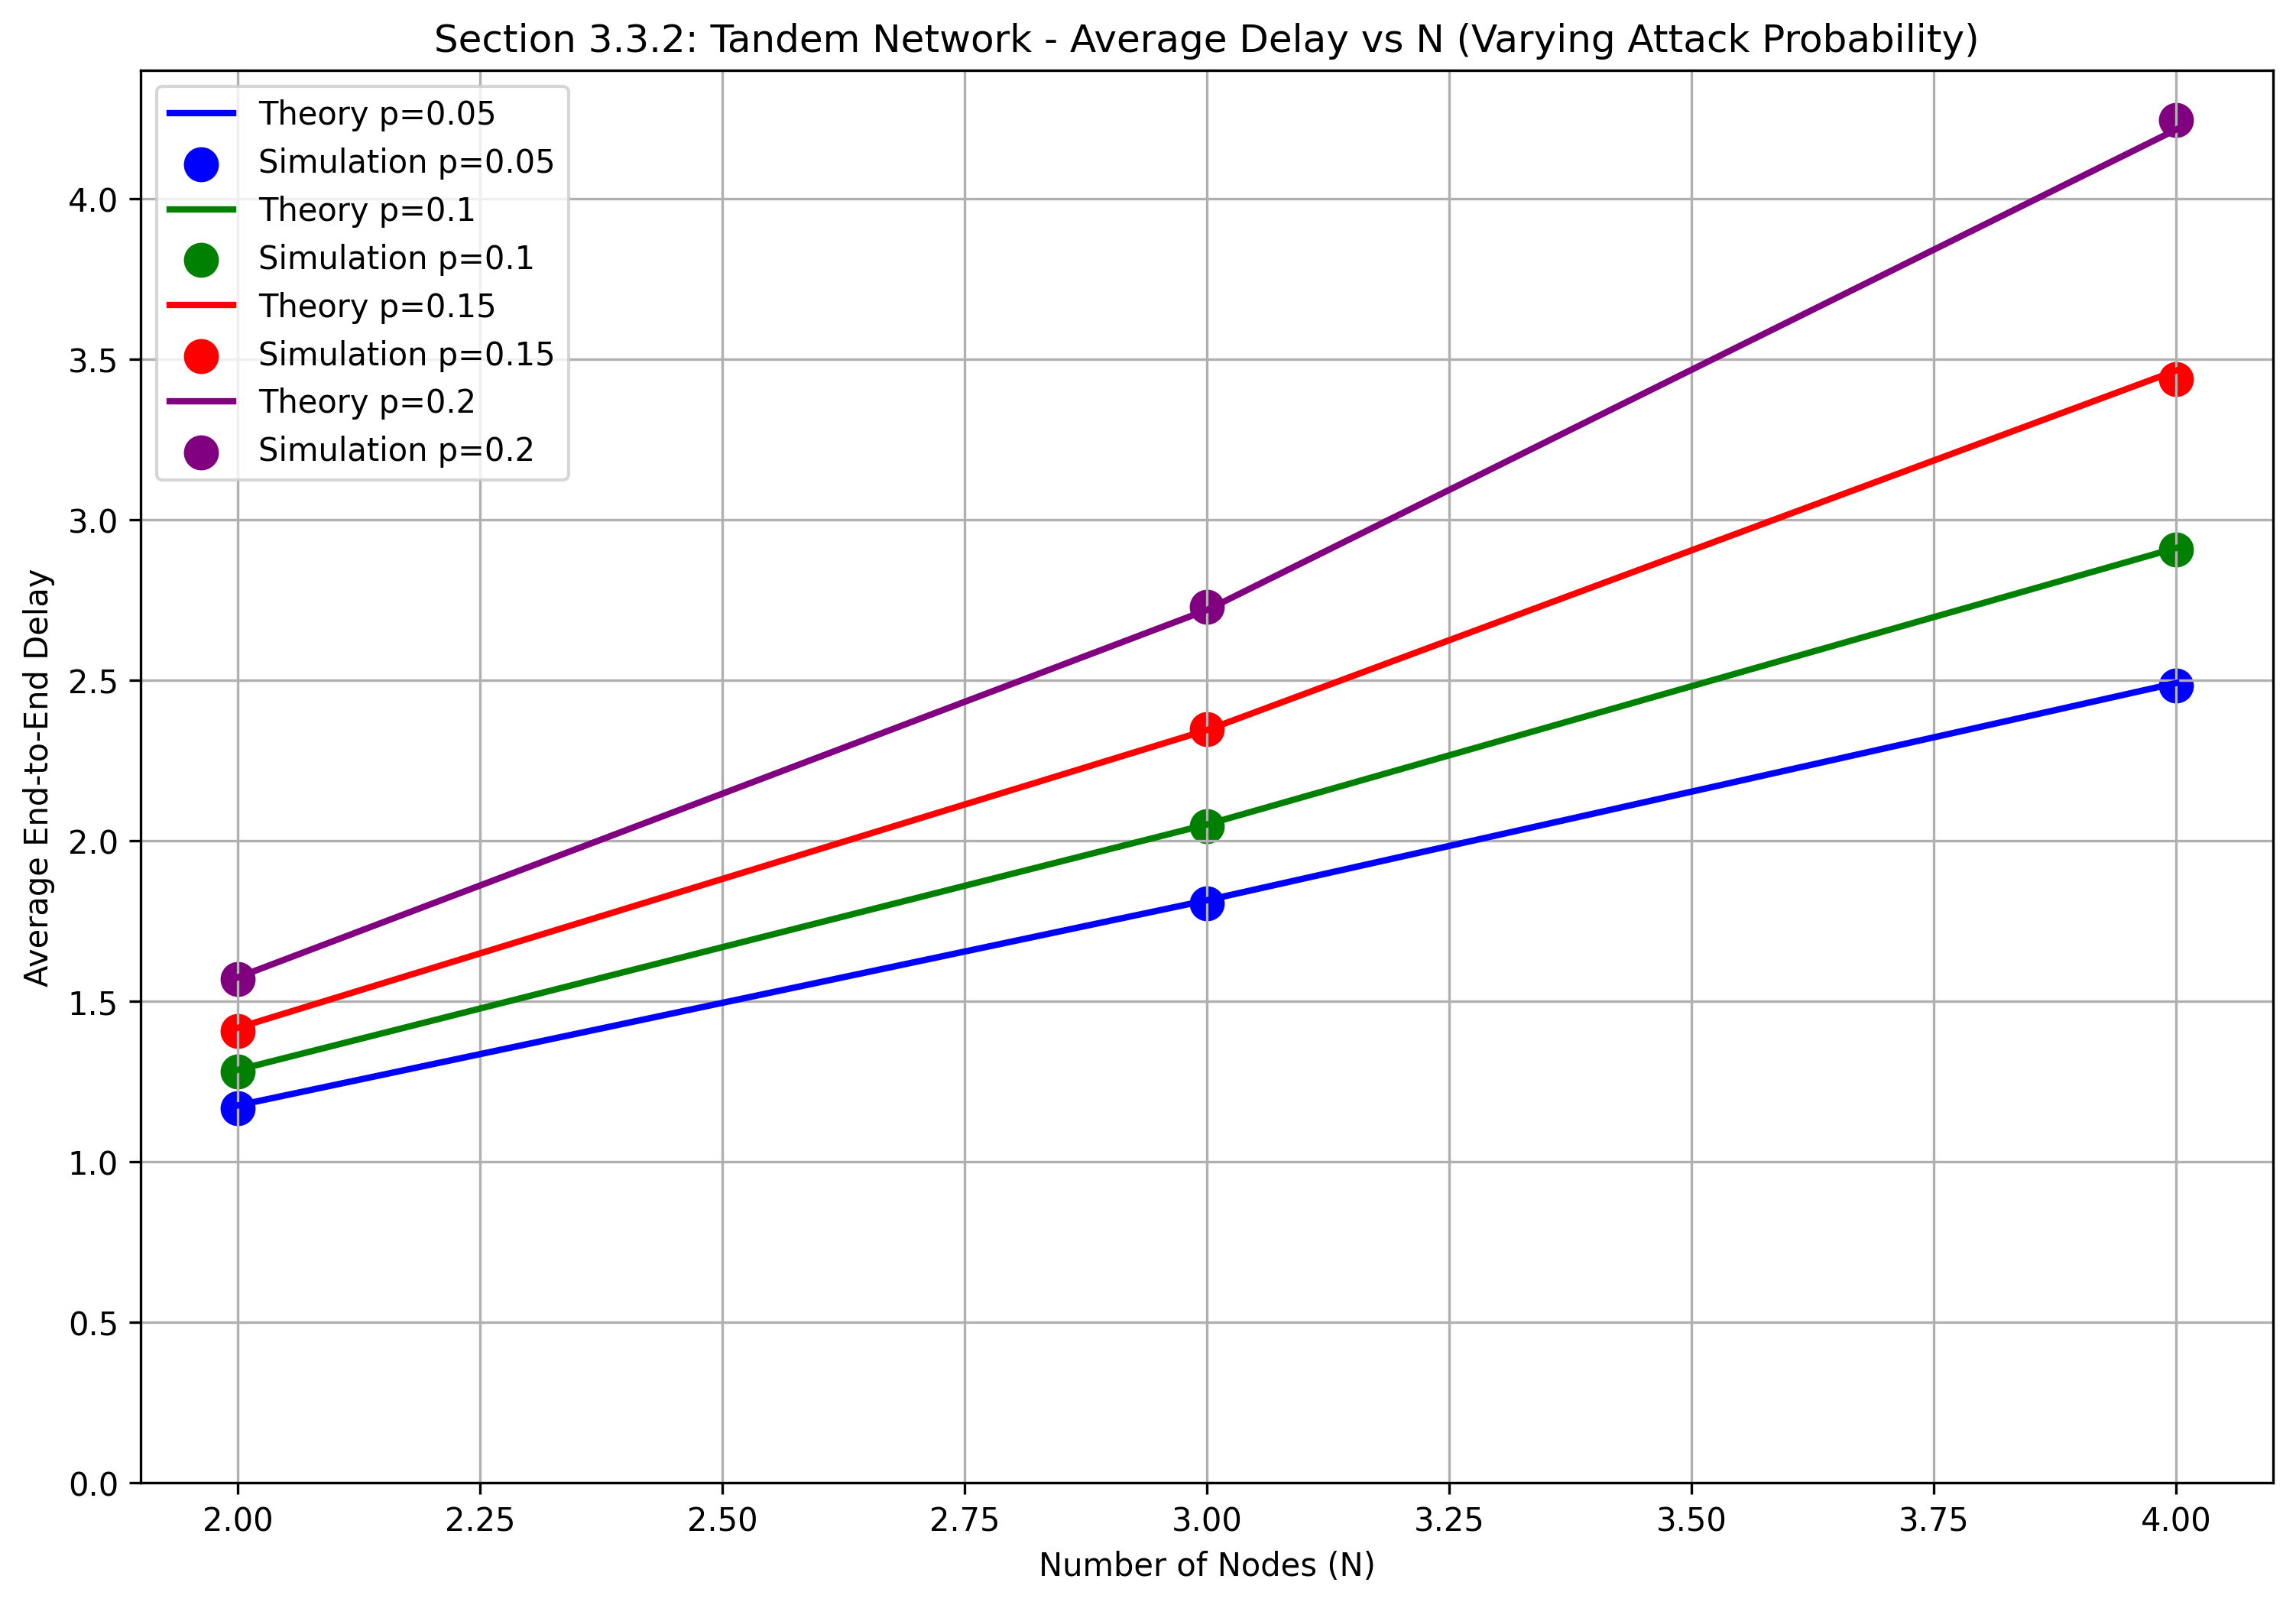
\includegraphics[width=\textwidth]{4_n_node_feedforward/section_3_3_2_tandem_delay_vs_N_varying_p.png}
        \caption{End-to-end delay vs. chain length $N$.}
        \label{fig:tandem}
    \end{subfigure}
    \hfill
    \begin{subfigure}[b]{0.48\textwidth}
        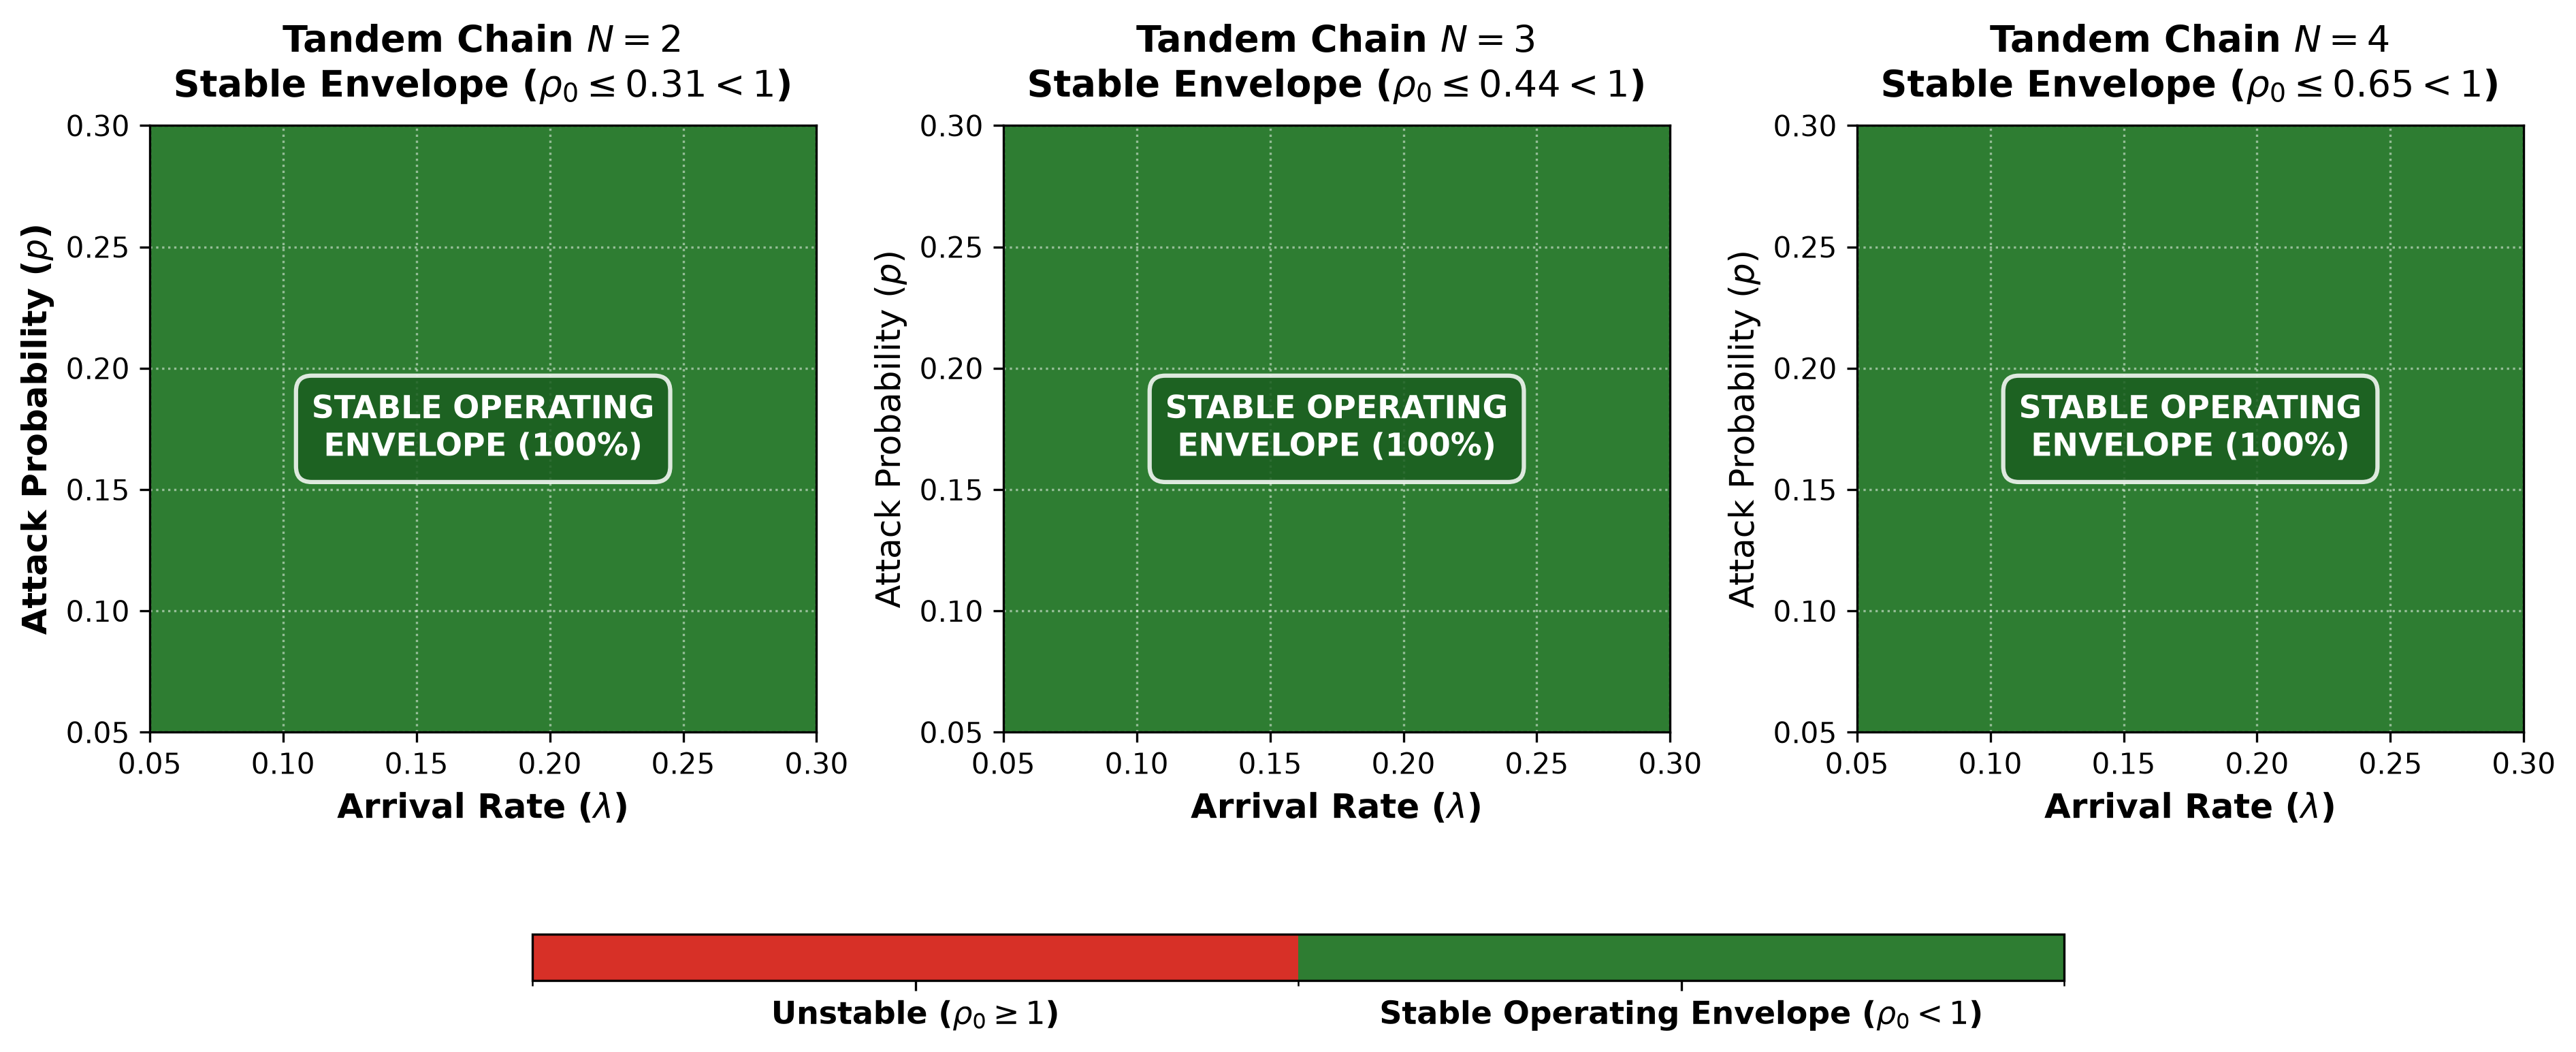
\includegraphics[width=\textwidth]{4_n_node_feedforward/section_3_3_2_stability_regions.png}
        \caption{Stability boundaries in $(\lambda, p)$ space.}
        \label{fig:stability}
    \end{subfigure}
    \caption{Multi-hop feedforward dynamics (Case 4). Left: Non-linear delay growth with $N$ across attack intensities. Right: Robust 100\% stable operating envelope across $(\lambda, p \in [0.05, 0.30])$ for $N \in \{2, 3, 4\}$.}
    \label{fig:tandem_combined}
\end{figure}

\section{Case Study 5: \texorpdfstring{$N$}{N}-Node Feedback Meshes}
\subsection{Topology, Routing Matrix, and Jackson Symmetry}
Consider an interconnected network of $N$ symmetric queueing nodes. External Poisson traffic arrives at each node $i \in \{0, \dots, N-1\}$ with rate $\lambda$ (total external arrival rate $N\lambda$). Each node has service rate $\mu$. Upon completing service at any node:
\begin{itemize}
    \item With probability $p$, the packet is attacked/corrupted, triggering an immediate failure and origin-based retransmission.
    \item With probability $1 - p$, the packet is intact.
    \begin{itemize}
        \item If total elapsed time from entry exceeds $W$, the packet times out and is retransmitted.
        \item Otherwise, with probability $q = \frac{1}{N+1}$, the packet exits the network successfully.
        \item With probability $1 - q = \frac{N}{N+1}$, the packet transitions uniformly to any of the $N$ nodes (transition probability $r_{ij} = \frac{1}{N+1}$ for all $j \in \{0, \dots, N-1\}$).
    \end{itemize}
\end{itemize}
By complete topological and traffic symmetry, all nodes maintain an identical total arrival rate $\Lambda^*$. The effective node clearance rate is:
\begin{equation}
\gamma = \mu - \Lambda^*
\end{equation}
The sojourn time per node visit is exponentially distributed: $X \sim \text{Exp}(\gamma)$.

\subsection{Erlang-\texorpdfstring{$k$}{k} Multi-Visit Sojourn Distribution}
The cumulative time required to complete $k$ successive node visits is the sum of $k$ independent $\text{Exp}(\gamma)$ random variables, which follows an \textbf{Erlang-$k$} distribution:
\begin{equation}
S_k = \sum_{j=1}^k X_j \sim \text{Erlang}(k, \gamma)
\end{equation}
The CDF of $S_k$ evaluated at the timeout window $W$ is:
\begin{equation}
F_k(W) = P(S_k \le W) = \frac{\gamma(k, \gamma W)}{\Gamma(k)} = 1 - \sum_{j=0}^{k-1} \frac{(\gamma W)^j e^{-\gamma W}}{j!}
\end{equation}
with the boundary convention $F_0(W) = 1$.

\subsection{Visit-by-Visit Probabilistic Decomposition}
A packet reaches visit $k \ge 1$ if it survived $k-1$ preceding visits without attack (probability $(1-p)^{k-1}$), chose internal transitions $k-1$ times (probability $(N/(N+1))^{k-1}$), and satisfied the timeout condition $S_{k-1} \le W$. Let $w_k \triangleq (1 - p)^{k-1}\left(\frac{N}{N+1}\right)^{k-1}$ denote the routing-survival weight and let the reach probability be:
\begin{equation}
u_k = w_k F_{k-1}(W) = (1 - p)^{k-1} \left(\frac{N}{N+1}\right)^{k-1} F_{k-1}(W)
\end{equation}
We derive the network metrics via infinite series expansions:
\begin{enumerate}
    \item \textbf{Expected Server Visits per Attempt $E[V]$:}
    \begin{equation}
    E[V] = \sum_{k=1}^\infty u_k = \sum_{k=1}^\infty (1 - p)^{k-1} \left(\frac{N}{N+1}\right)^{k-1} F_{k-1}(W)
    \end{equation}
    \item \textbf{Success Probability $P_{\text{succ}}$:} Success at visit $k$ requires escaping attack at visit $k$ (factor $1-p$), choosing network exit (factor $1/(N+1)$), and completing within timeout $W$ ($F_k(W)$):
    \begin{equation}
    P_{\text{succ}} = \sum_{k=1}^\infty P_{\text{succ}, k} = \sum_{k=1}^\infty (1 - p)^k \frac{N^{k-1}}{(N+1)^k} F_k(W)
    \end{equation}
    \item \textbf{Conditional Success Duration $E[D_{\text{succ}}]$:}
    \begin{equation}
    E[D_{\text{succ}}] = \frac{1}{P_{\text{succ}}} \sum_{k=1}^\infty P_{\text{succ}, k} \cdot E[S_k \mid S_k \le W] = \frac{1}{P_{\text{succ}}} \sum_{k=1}^\infty P_{\text{succ}, k} \left(\frac{k}{\gamma} \frac{F_{k+1}(W)}{F_k(W)}\right)
    \end{equation}
    \item \textbf{Failure Probabilities and Delay $E[D_{\text{fail}}]$:}
    \begin{itemize}
        \item Attack failure at visit $k$: $P_{\text{att}, k} = u_k \cdot p = w_k p F_{k-1}(W)$, with conditional duration $E[S_{k-1} + X_k \mid S_{k-1} \le W] = \frac{1}{\gamma} + \frac{k-1}{\gamma}\frac{F_k(W)}{F_{k-1}(W)}$.
        \item Timeout failure at visit $k$: $P_{\text{to}, k} = w_k (1 - p) [F_{k-1}(W) - F_k(W)]$, where $S_{k-1} \le W < S_k$; by the memoryless property of the $k$-th exponential visit $X_k \sim \text{Exp}(\gamma)$ across threshold $W$, its conditional duration is $E[S_k \mid S_{k-1} \le W < S_k] = W + \frac{1}{\gamma}$.
    \end{itemize}
    \begin{equation}
    E[D_{\text{fail}}] = \frac{\sum_{k=1}^\infty \left[ P_{\text{att}, k} \left(\frac{1}{\gamma} + \frac{k-1}{\gamma}\frac{F_k(W)}{F_{k-1}(W)}\right) + P_{\text{to}, k} \left(W + \frac{1}{\gamma}\right) \right]}{\sum_{k=1}^\infty (P_{\text{att}, k} + P_{\text{to}, k})}
    \end{equation}
    which satisfies the exact renewal-visit identity $P_{\text{succ}}E[D_{\text{succ}}] + (1 - P_{\text{succ}})E[D_{\text{fail}}] = E[V]/\gamma$.
\end{enumerate}

\subsection{Fixed-Point Traffic Equation and Delay}
Each external arrival generates an average of $E[V]/P_{\text{succ}}$ server visits across its entire lifecycle. By node symmetry, the fixed-point traffic balance at every node is:
\begin{equation}
\Lambda^* = \lambda \frac{E[V](\Lambda^*)}{P_{\text{succ}}(\Lambda^*)}
\label{eq:feedback_fixed_point}
\end{equation}
Solving Equation \eqref{eq:feedback_fixed_point} via damped Picard iteration yields $\Lambda^*$. The total end-to-end sojourn time is:
\begin{equation}
E[D] = \left(\frac{1}{P_{\text{succ}}} - 1\right) E[D_{\text{fail}}] + E[D_{\text{succ}}]
\end{equation}
Figure \ref{fig:feedback} illustrates the scaling of sojourn time with network size $N$. Unlike tandem chains, feedback meshes distribute retransmission load uniformly across all $N$ servers, yielding graceful and predictable delay scaling.

\begin{figure}[h]
    \centering
    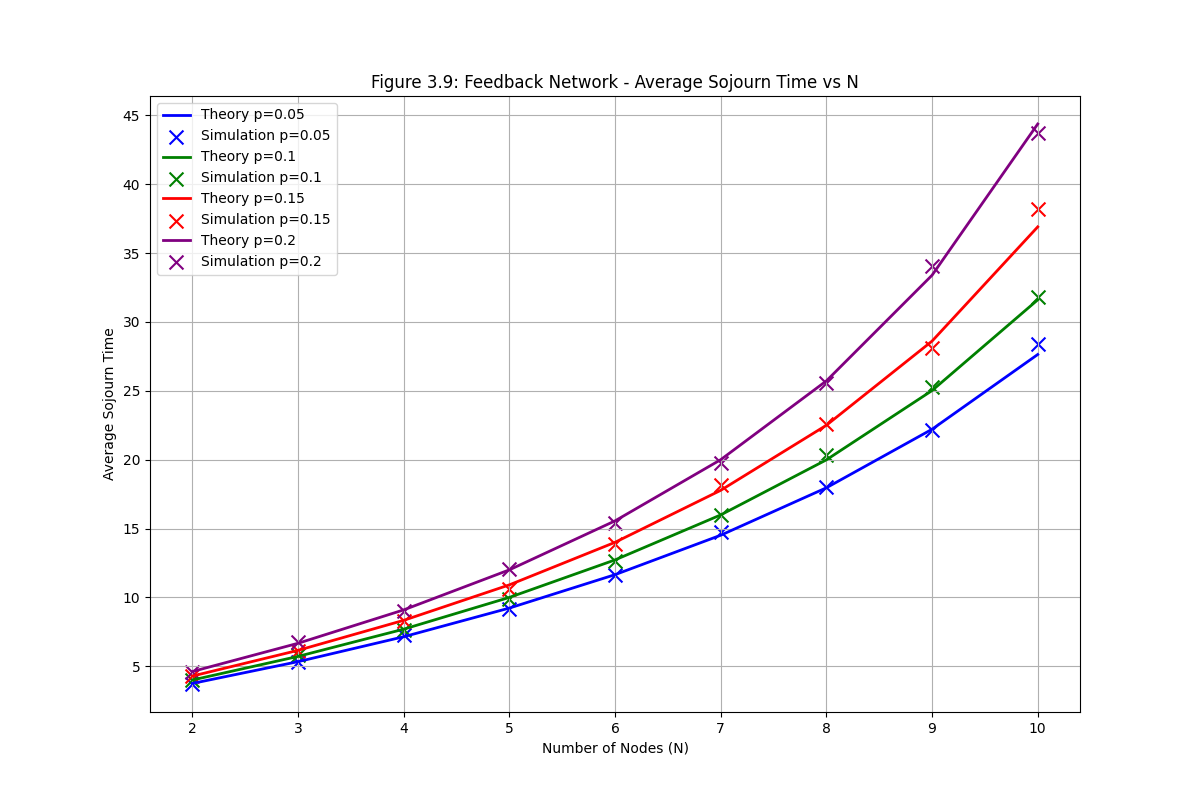
\includegraphics[width=0.75\textwidth]{5_n_node_feedback/section_3_3_1_sojourn_vs_N_varying_p.png}
    \caption{Case 5: End-to-end sojourn time in $N$-node feedback networks. Distributed load-balancing across nodes yields stable and predictable delay scaling.}
    \label{fig:feedback}
\end{figure}

\section{Comparative Theoretical Synthesis}
Table \ref{tab:theory_synthesis} provides a comprehensive synthesis of the theoretical formulations across all five case studies.

\begin{table}[ht]
\centering
\caption{Consolidated theoretical formulations across all five network case studies.}
{\scriptsize
\setlength{\tabcolsep}{2pt}
\begin{tabular*}{\textwidth}{@{\extracolsep{\fill}}lp{2.1cm}p{3.4cm}p{4.6cm}@{}}
\toprule
\textbf{Case Study} & \textbf{Effective Load $\rho$} & \textbf{Success Prob $P_{\text{succ}}$} & \textbf{End-to-End Delay $E[D]$} \\ \midrule
\textbf{Case 1: Destruction} & $\frac{\Lambda^*(1-p)}{\mu}$ & $(1-p)[1 - e^{-(\mu - \Lambda^*(1-p))T}]$ & $\frac{1}{P_{\text{succ}}}[E[W_q] + \frac{1-p}{\mu}] + (\frac{1}{P_{\text{succ}}}-1)B$ \\ \addlinespace
\textbf{Case 2: Modification} & $\frac{\Lambda^*}{\mu}$ & $(1-p)[1 - e^{-(\mu - \Lambda^*)T}]$ & $\frac{1}{P_{\text{succ}}(\mu - \Lambda^*)}$ \\ \addlinespace
\textbf{Case 3: 3-Node Tandem} & $\frac{\Lambda^*}{\mu}$ & $(1-p)^3 F_{\text{Erlang}}(W; 3, \mu-\Lambda^*)$ & $\frac{3}{P_{\text{succ}}(\mu - \Lambda^*)}$ \\ \addlinespace
\textbf{Case 4: General $N$-Tandem} & $\frac{\Lambda_0^*}{\mu}$ at Node 0 & $(1-p)^N P(k, W/\theta)$ & $(E[A]-1)E[D_{\text{fail}}] + \mu_S \frac{P(k+1, W/\theta)}{P(k, W/\theta)}$ \\ \addlinespace
\textbf{Case 5: $N$-Node Feedback} & $\frac{\lambda E[V]}{\mu P_{\text{succ}}}$ & $\sum_{k=1}^\infty (1-p)^k \frac{N^{k-1}}{(N+1)^k} F_k(W)$ & $(E[A]-1)E[D_{\text{fail}}] + \frac{1}{P_{\text{succ}}}\sum_k P_{\text{succ}, k}\frac{k}{\gamma}\frac{F_{k+1}(W)}{F_k(W)}$ \\ \bottomrule
\end{tabular*}}
\label{tab:theory_synthesis}
\end{table}

\section{Experimental Validation}
The proposed analytical models were validated against discrete-event simulations implemented in SimPy~\cite{matloff2008introduction}. Simulations were executed with 200 replications, a warm-up period of 2,000 time units, and an active observation horizon of 20,000 time units per replication. 

\begin{table}[ht]
\centering
\caption{Cross-validation of analytical models vs. high-fidelity SimPy simulations.}
{\scriptsize
\setlength{\tabcolsep}{1.5pt}
\begin{tabular*}{\textwidth}{@{\extracolsep{\fill}}lp{5.0cm}cccc@{}}
\toprule
\textbf{Scenario} & \textbf{Parameters} & \textbf{Theory (s)} & \textbf{Sim (s)} & \textbf{Gap} & \textbf{Err. (\%)} \\ \midrule
\textbf{Case 1: Destruction} & $N=1, \mu=10, \lambda=1.44, p=0.2, W=2, B=0.03$ & 0.1286 & 0.1261 & 0.0025 & 1.91\% \\
\textbf{Case 2: Modification} & $N=1, \mu=10, \lambda=1.44, p=0.2, W=2$ & 0.1525 & 0.1523 & 0.0002 & 0.15\% \\
\textbf{Case 3: 3-Node Tandem} & $N=3, \mu=2.0, \lambda=0.15, p=0.10, W=8$ & 2.2938 & 2.2965 & 0.0027 & 0.12\% \\
\textbf{Case 4: Feedforward} & $N=4, \mu=2.0, \lambda=0.15, p=0.10, W=8$ & 2.9124 & 2.9079 & 0.0045 & 0.15\% \\
\textbf{Case 5: Feedback Mesh} & $N=10, \mu=1.0, \lambda=0.05, p=0.10, W=50$ & 31.8883 & 31.8035 & 0.0848 & 0.27\% \\ \bottomrule
\end{tabular*}}
\label{tab:validation}
\end{table}

As shown in Table \ref{tab:validation}, the theoretical predictions align closely with the simulation data across all five case studies, with relative errors remaining below 2\% in all regimes and strictly under 0.30\% for multi-node networks. Under identical workload parameters ($N=1, \mu=10, \lambda=1.44, p=0.2$), modification attacks induce an 18.6\% delay surge over destruction attacks ($0.1525$\,s vs.\ $0.1286$\,s) due to wasted server cycles. The maximum multi-node error is 0.27\% (in the 10-node feedback mesh).

\section{Saddle-Node Retry Bifurcation and Critical Collapse Theory}
\label{sec:bifurcation}
While the classical stability boundary $\rho < 1$ governs open queues without timeout-driven retransmissions, an adversarial queue with finite timeout $T$ and attack rate $p$ under the mean-field renewal-conservation closure obeys the nonlinear map:
\begin{equation}
\Gamma(\Lambda^*; p, \mu, T) \triangleq \Lambda^* \tilde{P}_{\text{succ}}(\Lambda^*; p, \mu, T) = \lambda,
\label{eq:conservation_map}
\end{equation}
where $\Lambda^* \in (0, \Lambda_{\max})$ is the bottleneck internal attempt rate and $\tilde{P}_{\text{succ}}(\Lambda^*)$ equals $P_{\text{succ}}(\Lambda^*)$ for Cases~1--4 and the per-visit exit yield $P_{\text{succ}}(\Lambda^*)/E[V](\Lambda^*)$ for Case~5 (Eq.~\ref{eq:feedback_fixed_point}). Because $\Gamma(0) = \Gamma(\Lambda_{\max}) = 0$ and $\Gamma(\Lambda^*) > 0$ on $(0, \Lambda_{\max})$, $\Gamma(\Lambda^*)$ attains an interior fold maximum $(\Lambda_{\text{SN}}^*, \lambda_{\text{crit}}^{\text{SN}})$ where a \textbf{Saddle-Node (Fold) Retry Bifurcation}~\cite{strogatz2015nonlinear} occurs under the quasi-stationary relaxation dynamics $\dot{\Lambda} = \kappa_r[\lambda - \Gamma(\Lambda)]$.

\subsection{Closed-Form Wright-\texorpdfstring{$\omega$}{omega} / Lambert-\texorpdfstring{$W_0$}{W0} Fold Theorem}
For Case 2 (Post-Service Modification), $\Gamma_{\text{mod}}(\Lambda^*) = (1 - p)\Lambda^*(1 - e^{-(\mu - \Lambda^*)T})$ is strictly concave on $[0, \mu]$:
\begin{equation}
\frac{\partial^2 \Gamma_{\text{mod}}}{\partial (\Lambda^*)^2} = -(1 - p)T(2 + \Lambda^* T)e^{-(\mu - \Lambda^*)T} < 0.
\end{equation}
Setting $\partial \Gamma_{\text{mod}}/\partial \Lambda^* = (1 - p)[1 - (1 + \Lambda^* T)e^{-(\mu - \Lambda^*)T}] = 0$ and substituting $v = 1 + \Lambda^* T > 1$ yields the transcendental equation $v e^v = e^{\mu T + 1}$, which admits an exact closed-form solution in terms of the principal Lambert-$W_0$ branch~\cite{corless1996lambertw} and the Wright $\omega$ function $\omega(z) = W_0(e^z)$:
\begin{equation}
\Lambda_{\text{SN}}^{\text{mod}}(\mu, T) = \frac{\omega(\mu T + 1) - 1}{T}, \qquad
\lambda_{\text{crit}}^{\text{SN,mod}}(p, \mu, T) = \frac{1 - p}{T}\frac{[\omega(\mu T + 1) - 1]^2}{\omega(\mu T + 1)}.
\label{eq:wright_omega_sn}
\end{equation}
Evaluating the second derivative at $e^{-(\mu - \Lambda_{\text{SN}}^*)T} = 1/\omega(\mu T + 1)$ gives the exact quadratic normal-form curvature $c_2 = -\frac{1}{2}\Gamma_{\text{mod}}''(\Lambda_{\text{SN}}^*)$:
\begin{equation}
c_2^{\text{mod}}(p, \mu, T) = \frac{(1 - p)\,T\,[1 + \omega(\mu T + 1)]}{2\,\omega(\mu T + 1)} > 0.
\label{eq:normal_form_c2}
\end{equation}
For the multi-hop topologies, $\Gamma_{\text{tandem}}(\Lambda^*)$ (Case~3), $\Gamma_{\text{ff}}(\Lambda_0^*)$ with stage attenuation $\Lambda_i^* = \Lambda_0^*(1-p)^i$ and Gamma moment-matching (Case~4), and $\Gamma_{\text{fb}}(\Lambda^*) = \Lambda^* P_{\text{succ}}(\Lambda^*)/E[V](\Lambda^*)$ (Case~5) are maximized numerically on $(0, \mu)$. Because stage attenuation unloads downstream nodes $i \ge 1$ in Case~4 relative to symmetric Case~3, Case~4 sustains a strictly higher fold attempt rate and critical throughput ($\Lambda_{\text{SN}}^{\text{ff}} = 7.3034 > \Lambda_{\text{SN}}^{\text{tandem}} = 6.7316$ and $\lambda_{\text{crit}}^{\text{SN,ff}} = 3.4780 > \lambda_{\text{crit}}^{\text{SN,tandem}} = 3.1713$ at $N=2, \mu=10, T=1, p=0.25$).

\subsection{Structural \texorpdfstring{$p$}{p}-Invariance of Pre-Service Destruction vs.\ Modification Erosion}
A fundamental structural dichotomy emerges between Case 1 (Pre-Service Destruction) and Case 2 (Post-Service Modification). Under pre-service destruction, only surviving traffic $x \triangleq (1 - p)\Lambda^* \in (0, \mu)$ enters the server, so the conservation map reduces to a function of $x$ alone:
\begin{equation}
\Gamma_{\text{dest}}(\Lambda^*; p, \mu, T) = x\!\left(1 - e^{-(\mu - x)T}\right) \triangleq G_{\text{dest}}(x; \mu, T).
\label{eq:dest_invariance}
\end{equation}
Differentiating Eq.~\eqref{eq:dest_invariance} with respect to $p$ at fixed effective server load $x$ yields $\partial G_{\text{dest}}/\partial p \equiv 0$. Consequently, the critical external throughput capacity $\lambda_{\text{crit}}^{\text{SN,dest}}(\mu, T) = [\omega(\mu T + 1) - 1]^2 / [T\omega(\mu T + 1)]$ is \textbf{strictly invariant to the attack probability} $p \in [0, 1)$ and coincides identically with $\lambda_{\text{crit}}^{\text{SN,mod}}(0, \mu, T)$ at $p = 0$, whereas the internal attempt rate at the fold scales inversely as $\Lambda_{\text{SN}}^{\text{dest}}(p) = [\omega(\mu T + 1) - 1]/[(1 - p)T]$ with curvature $c_2^{\text{dest}}(p) = (1-p)^2 T[1 + \omega(\mu T + 1)]/[2\omega(\mu T + 1)]$. Conversely, under post-service modification, corrupted packets consume full service cycles before detection, causing $\lambda_{\text{crit}}^{\text{SN,mod}}(p) = (1 - p)\lambda_{\text{crit}}^{\text{SN,mod}}(0)$ to erode linearly to zero as $p \to 1$, with critical attack threshold $p_{\text{crit}}^{\text{SN,mod}}(\lambda) = 1 - \lambda / \lambda_{\text{crit}}^{\text{SN,mod}}(0)$.

\subsection{Dual Fixed-Point Branches, Separatrix Gap, and Square-Root Critical Exponent}
Under the mean-field renewal closure, for every subcritical arrival rate $\lambda \in (0, \lambda_{\text{crit}}^{\text{SN}})$, Eq.~\eqref{eq:conservation_map} admits two fixed points:
\begin{enumerate}
    \item A \textbf{locally stable lower branch} $\Lambda_{\text{stable}}^*(\lambda) \in (0, \Lambda_{\text{SN}}^*)$ where $\Gamma'(\Lambda_{\text{stable}}^*) > 0$, and
    \item A \textbf{locally unstable upper branch (separatrix)} $\Lambda_{\text{unstable}}^*(\lambda) \in (\Lambda_{\text{SN}}^*, \Lambda_{\max})$ where $\Gamma'(\Lambda_{\text{unstable}}^*) < 0$,
\end{enumerate}
which coalesce into a marginally semistable fold point at $\lambda = \lambda_{\text{crit}}^{\text{SN}}$. As $\lambda \uparrow \lambda_{\text{crit}}^{\text{SN}}$, expanding $\Gamma(\Lambda^*)$ around $\Lambda_{\text{SN}}^*$ yields the quadratic normal form $\lambda_{\text{crit}}^{\text{SN}} - \lambda = c_2(\Lambda^* - \Lambda_{\text{SN}}^*)^2 + \mathcal{O}(|\Lambda^* - \Lambda_{\text{SN}}^*|^3)$, so the separatrix stability margin $\Delta\Lambda_{\text{sep}}(\lambda) \triangleq \Lambda_{\text{unstable}}^*(\lambda) - \Lambda_{\text{stable}}^*(\lambda)$ vanishes with a square-root singularity:
\begin{equation}
\Lambda_{\text{unstable}}^*(\lambda) - \Lambda_{\text{stable}}^*(\lambda) = 2\sqrt{\frac{\lambda_{\text{crit}}^{\text{SN}} - \lambda}{c_2}} + \mathcal{O}(\lambda_{\text{crit}}^{\text{SN}} - \lambda), \qquad
\frac{\partial \Lambda_{\text{stable}}^*}{\partial \lambda} \sim \frac{1}{2\sqrt{c_2(\lambda_{\text{crit}}^{\text{SN}} - \lambda)}}.
\label{eq:sqrt_scaling}
\end{equation}
In a finite-backoff stochastic queue, $\Lambda_{\text{stable}}^*(\lambda)$ is metastable: either a transient adversarial burst or an endogenous queue-length fluctuation across the shrinking barrier $\Delta\Lambda_{\text{sep}}(\lambda)$ drives the system across $\Lambda_{\text{unstable}}^*(\lambda)$ into runaway timeout amplification even when $\lambda < \lambda_{\text{crit}}^{\text{SN}}$. Figure~\ref{fig:saddle_node_bifurcation} and Table~\ref{tab:bifurcation_summary} summarize the bifurcation invariants across all five topologies.

\begin{figure}[ht]
    \centering
    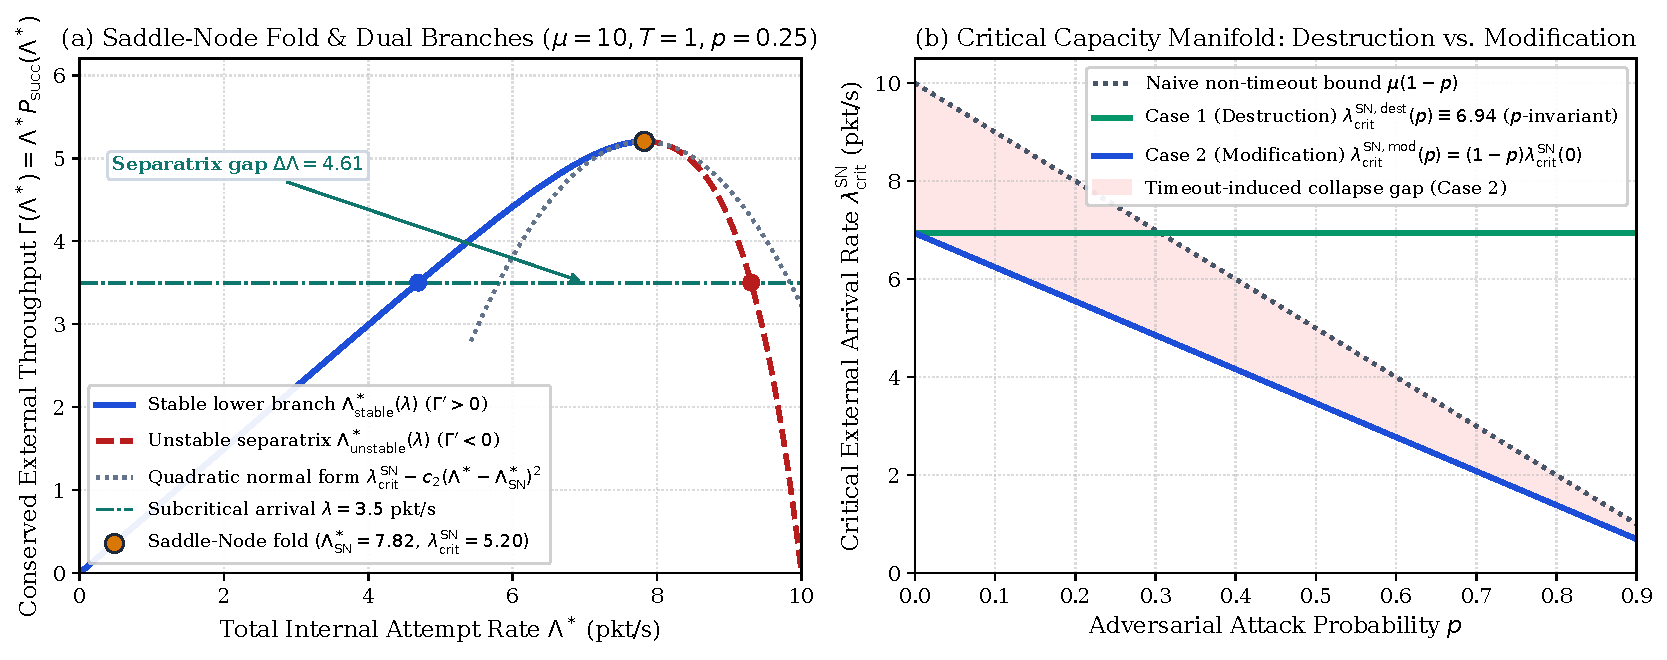
\includegraphics[width=0.98\textwidth]{fig_saddle_node_bifurcation.pdf}
    \caption{Saddle-Node retry bifurcation analysis ($\mu=10, T=1, p=0.25$): (a) unimodal throughput conservation curve $\Gamma(\Lambda^*)$ showing the stable lower branch $\Lambda_{\text{stable}}^*$, unstable upper separatrix $\Lambda_{\text{unstable}}^*$, Wright-$\omega$ fold point $(\Lambda_{\text{SN}}^*=7.82, \lambda_{\text{crit}}^{\text{SN}}=5.20)$, and quadratic normal form; (b) critical capacity manifold $\lambda_{\text{crit}}^{\text{SN}}(p)$ contrasting Case~1 structural $p$-invariance ($\equiv 6.94$) against Case~2 linear capacity erosion.}
    \label{fig:saddle_node_bifurcation}
\end{figure}

\begin{table}[ht]
\centering
\caption{Saddle-Node (Fold) retry bifurcation invariants across all five topologies ($\mu=10, T=1, p=0.25, N=2$).}
{\scriptsize
\setlength{\tabcolsep}{2pt}
\begin{tabular*}{\textwidth}{@{\extracolsep{\fill}}lcccccc@{}}
\toprule
\textbf{Topology} & \textbf{Fold $\Lambda_{\text{SN}}^*$} & \textbf{Crit.\ $\lambda_{\text{crit}}^{\text{SN}}$} & \textbf{Util.\ $\rho_{\text{SN}}$} & \textbf{Curv.\ $c_2$} & \textbf{Naive Cap.} & \textbf{Cap.\ Ratio} \\ \midrule
\textbf{Case 1: Destruction} & 10.4302 & 6.9360 & 0.7823 & 0.3131 & 10.0000 & 69.36\% \\
\textbf{Case 2: Modification} & 7.8227 & 5.2020 & 0.7823 & 0.4175 & 7.5000 & 69.36\% \\
\textbf{Case 3: Tandem ($N=2$)} & 6.7316 & 3.1713 & 0.6732 & 0.2335 & 5.6250 & 56.38\% \\
\textbf{Case 4: Feedforward ($N=2$)} & 7.3034 & 3.4780 & 0.7303 & 0.2373 & 5.6250 & 61.83\% \\
\textbf{Case 5: Feedback ($N=2$)} & 7.6389 & 1.5633 & 0.7639 & 0.0965 & 2.5000 & 62.53\% \\ \bottomrule
\end{tabular*}}
\label{tab:bifurcation_summary}
\end{table}

\section{Conclusion}
This paper presented a rigorous mathematical theory for evaluating packet sojourn time, Saddle-Node retry bifurcations, and network stability across five distinct topologies under active adversarial attacks and timeout-driven retransmissions. By formulating exact renewal-reward equations, closed-form Wright-$\omega$ / Lambert-$W_0$ fold thresholds for single-node destruction and modification, multi-hop hypoexponential moment-matching, stage-wise traffic attenuation, and Erlang visit summations, we demonstrated that retransmissions induce non-linear traffic amplification loops and metastable separatrix boundaries that fundamentally govern system capacity. High-fidelity discrete-event simulations across all five topologies and symbolic computer-algebra proofs for the single-node Wright-$\omega$ fold theorems confirmed the accuracy of the analytical models.

\begin{thebibliography}{99}
\bibitem{kleinrock1975queueing}
L.~Kleinrock, \textit{Queueing Systems, Volume 1: Theory}, Wiley-Interscience, New York, 1975.

\bibitem{kleinrock1976computer}
L.~Kleinrock, \textit{Queueing Systems, Volume 2: Computer Applications}, John Wiley \& Sons, New York, 1976.

\bibitem{ross1996stochastic}
S.~M.~Ross, \textit{Stochastic Processes}, 2nd~ed., John Wiley \& Sons, New York, 1996.

\bibitem{jackson1957networks}
J.~R.~Jackson, ``Networks of waiting lines,'' \textit{Operations Research}, vol.~5, no.~4, pp.~518--521, 1957.

\bibitem{burke1956output}
P.~J.~Burke, ``The output of a queuing system,'' \textit{Operations Research}, vol.~4, no.~6, pp.~699--704, 1956.

\bibitem{cox1955use}
D.~R.~Cox, ``A use of complex probabilities in the theory of stochastic processes,'' \textit{Mathematical Proceedings of the Cambridge Philosophical Society}, vol.~51, no.~2, pp.~313--319, 1955.

\bibitem{altiok1985approximate}
T.~Altiok, ``On the phase-type approximations of general distributions,'' \textit{IIE Transactions}, vol.~17, no.~2, pp.~110--116, 1985.

\bibitem{pelechrinis2011denial}
K.~Pelechrinis, M.~Iliofotou, and S.~V.~Krishnamurthy, ``Denial of service attacks in wireless networks: The case of jammers,'' \textit{IEEE Communications Surveys \& Tutorials}, vol.~13, no.~2, pp.~245--257, 2011.

\bibitem{wood2002denial}
A.~D.~Wood and J.~A.~Stankovic, ``Denial of service in sensor networks,'' \textit{IEEE Computer}, vol.~35, no.~10, pp.~54--62, 2002.

\bibitem{fall1996simulation}
K.~Fall and S.~Floyd, ``Simulation-based comparisons of Tahoe, Reno, and SACK TCP,'' \textit{ACM SIGCOMM Computer Communication Review}, vol.~26, no.~3, pp.~5--21, 1996.

\bibitem{matloff2008introduction}
N.~Matloff, ``Introduction to discrete-event simulation and the SimPy language,'' \textit{Dept. of Computer Science, University of California, Davis}, 2008.

\bibitem{corless1996lambertw}
R.~M.~Corless, G.~H.~Gonnet, D.~E.~G.~Hare, D.~J.~Jeffrey, and D.~E.~Knuth, ``On the Lambert $W$ function,'' \textit{Advances in Computational Mathematics}, vol.~5, no.~1, pp.~329--359, 1996.

\bibitem{strogatz2015nonlinear}
S.~H.~Strogatz, \textit{Nonlinear Dynamics and Chaos: With Applications to Physics, Biology, Chemistry, and Engineering}, 2nd~ed., Westview Press, Boulder, CO, 2015.
\end{thebibliography}

\section*{About the Author}
\noindent\textbf{Ilias Chrysovergis} is with the Department of Electrical and Electronic Engineering, Imperial College London, and Metatopia. His research interests encompass distributed systems, communication network resilience, stochastic queueing theory, and security protocol engineering in adversarial environments. E-mail: \texttt{ilias@chrysovergis.gr}.

\end{document}
